\chapter{持续集成} % Introduction chapter suppressed from the table of contents

Thomas先生的“每小步验证”原则,开发大型复杂系统,都应先拆分子系统/模块,先开发并测试子系统/模块、集成再测试,这样按部就班地完成整个系统的开发。

\hypertarget{ux9a8cux6536ux6d4bux8bd5}{%
\subsection{验收测试}\label{ux9a8cux6536ux6d4bux8bd5}}

验收要满足需求,需求要可验证,所以,通过相应需求的测试成为验收通过的必要条件。
需求确定后,就可以规范验收通过的准则,开始准备验收测试了。

很多QA人员理解验收测试为只做黑盒测试:

\begin{itemize}
\tightlist
\item
  把开发出来的系统看成一个黑盒,开发人员已经做好本身的所有自测(包括单元测试集成测试等),然后系统要通过我们的系统测试用例,包括功能与非功能。
\end{itemize}

\hypertarget{ux5e38ux89c1ux95eeux9898}{%
\subsubsection{常见问题}\label{ux5e38ux89c1ux95eeux9898}}

当开发人员完成了所有模块的开发,开始进行系统测试的时候,往往已经到了项目(或迭代)交付预期的后期, 这时如果发现大量缺陷,开发人员没有时间做好修复,即便修复后,也没有充足的时间做回归测试(重新跑本来通过的测试用例,确保不会因为开发人员的修改,而引起新的错误。)

\hypertarget{ux6539ux5584ux65b9ux6cd5}{%
\subsubsection{改善方法}\label{ux6539ux5584ux65b9ux6cd5}}

要避免这种恶性循环,减少发布延期的概率,
QA/测试人员就要参考前面预先排除缺陷,以降低质量成本的概念,尽早在项目的前期暴露缺陷并及时解决,不要等到系统测试时才处理。
所以不能单靠开发人员自觉做单元测试/集成测试。

\framebox{%
\begin{minipage}[t]{0.97\columnwidth}\raggedright
从开发人员的视角,他不会想主动用测试找出问题

最佳场景:开发完成,交给系统测试,没有被发现缺陷, 通过,结束。

再开发新的模块。

“精明”的编码人员思路:“如果对测试/缺陷没有要求,多严峻的开发进度目标,我都能轻易达成。”\strut
\end{minipage}}

所以要做好验收测试,QA/测试人员不仅仅是做最后的黑盒系统测试,而是要从单元测试开始,设定好测试通过准则
(Definition of Done
DoD),然后交给开发人员执行,要看到所有测试,从单元测试开始,都完全通过,才算通过验收,
才能避免上面的问题。(如果QA/测试人员的技术能力有限,起码要明确所有测试的准则(测试用例))

反之,QA/测试人员仅做最后黑盒测试,不能按时交付/交付质量问题,始终难以解决。

测试策略小建议:

\begin{enumerate}
\tightlist
\item
  在项目一开始便要开始写测试用例(在设计、编码之前)
\item
  代码每次有任何变动时,利用持续集成系统自动跑测试
\item
  有了自动化就可以轻松实现回归测试
\item
  以上不仅仅是覆盖功能测试,也包括非功能,例如安全性、性能负载量等
\end{enumerate}

目的:尽早让开发人员获得反馈,以此驱动他们能随时达到一个可发布的状态。\\
自动化让测试人员可以集中精力针对一些特有的测试,减少重复性测试的工作量。

\hypertarget{ux6d4bux8bd5ux81eaux52a8ux5316}{%
\subsection{测试自动化}\label{ux6d4bux8bd5ux81eaux52a8ux5316}}

\framebox{%
\begin{minipage}[t]{0.97\columnwidth}\raggedright
与设计开发人员探讨他们的产品集成过程:\\问:你们有没有用一些自动集成的工具,例如Jenkins集成工作自动化,原因是集成很花时间,现在也越来越流行持续集成、每天集成,所以如果靠手工集成、打包是很花工作量的。\\ 答:没有,我们还是手工。\\问:你们在手工集成之前怎么确保这些模块已经可以?\\ 答:我们有测试。\\ 问:做什么测试,可否举些例子?\\答:我们开发完以后,会输入一些查询,然后看是否能正常使用。\\ 问:我不是指整个系统功能的测试。例如,要通过你们java开发,有自动化单元测试,可以写脚本,如果你单元测试通过,就变绿,不然的话就红,你们有做吗?\\答:没有,我们都是手工测试。其实我们现在到了产品升级、增加功能的维护期了,记得在当初首次开发的时候,我们开发人员是有用Jenkins自动化集成,但现在维护期我们就没有。\strut
\end{minipage}}

从以上对话,可以了解到很多开发维护团队,基本就没有再做一步一步集成的过程,只是针对修改的功能,开发完就测试一下,然后便交到系统测试。

如果只是依靠对整个系统的集成测试:

\begin{itemize}
\tightlist
\item
  不一定能找到所有问题。当我们改动了一些代码,却没有通过模块的单元测试,就很难确保模块的每一次改动都是正确的。所以,这将导致如果后续确有问题的话,就很难定位或者难以修复
\item
  如果没有单元测试的话,你其实是不敢改动代码的,不知道改完以后对不对?
\end{itemize}

所以单元测试很重要,也因为单元测试高复用度,所以需要自动化才能节省大量手工测试工作量。\\
集成的概念,就是先写自动化单元测试用例,然后才写代码。通过单元测试才可以进入下一步集成测试,两个模块之间是否通。到最后进行总的系统测试,一步一步去做。如果团队像刚才那种情况,绕过了那些步骤,直接做总系统或集成测试。就可能会有很多隐患,到最终的验收测试才被发现,付出大量的缺陷修复代价。产品集成很重要,很花时间,所以绝大部分的团队如果注重软件质量的话,都会把产品集成自动化。改了代码之后,每天靠脚本来通过单元测试,比如它晚上自动跑产品集成发现的问题,第二天暴露给开发人员修改,修改后再集成看看有没有问题出现。有些公司除了要求单元测试通过以外,也会要求通过代码的静态扫描,道理都一样。只有用这种一层一层进行产品集成的方式,才可以有效确保软件的质量。正如Cunningham , Fowler等敏捷大师所说,没有做好集成过程里的测试会产生很多债务,产品交付给客户以后,因为质量问题导致还债的代价就更高。(详见附件某技术债务例子)

\hypertarget{ux6301ux7eedux96c6ux6210-continuous-integration}{%
\subsection{持续集成 Continuous
Integration}\label{ux6301ux7eedux96c6ux6210-continuous-integration}}

持续集成的道理很简单,每次提交代码做的修改,系统都可以自动构建整个系统,并跑通相关的自动化测,如果发现自动构建出错必须立马停下来修改缺陷。
团队要开始持续集成,起码要具备以下三个条件:

\begin{enumerate}
\tightlist
\item
  版本管理:所有的代码测试脚本、数据库脚本/构建脚本等都放在一个版本的管理系统管理,不仅仅是代码
\item
  利用工具实现自动构建( e.g. Jenkins
  ),虽然很多IDE集成开发环境都有这方面的功能,我们建议还是要用命令式(command)去跑构建脚本(像跑程序一样),每一次构建都能有详细记录(也随时可以重跑)
\item
  持续集成不仅仅依赖工具自动化,还需要整个团队高度付出、参与和自律,每个人频繁以每个小步交付他的开发部分。James
  SHORE 先生在 "Continuous integration on a dollar a
  day"文章里提出不一定依赖自动集成工具(e.g. CruiseControl 另一种类似
  Jenkins的集成工具 )
  只要每个团队成员都做好自动化单元测试,每次提交代码都使用版本管理系统合并,
  也能做到持续集成
\end{enumerate}

%\href{文件:!DeployPipelineScreenshot_2022-05-20_210104.jpg}{600px}

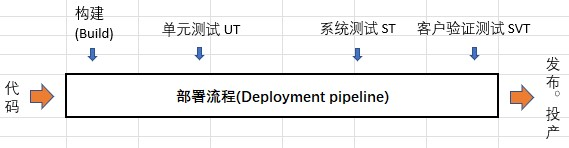
\includegraphics[width=10cm]{!DeployPipelineScreenshot_2022-05-20_210104.jpg}

不要以为每个开发人员每天提交(commit)代码到版本管理系统就算做到持续集成了,
还需要:

\begin{itemize}
\tightlist
\item
  每次提交代码要确保已经测试过,没有问题
\item
  所有部署发布后的问题都能在10分钟之内解决
\end{itemize}

不然就不算达到持续集成的基本条件。所以每天提交只是持续集成的第一步。

所以要做到持续集成得符合以下三个条件:

\begin{enumerate}
\tightlist
\item
  是否频繁把变更更新到主干去
\item
  有没有对应的自动化测试,确保集成后的代码是能通过所有测验
\item
  如果构建失败不能通过测试,必须立马停下修正代码,直到测试通过。有人会质疑为什么要这么频繁去更新主干的代码,自己分析测试好不也一样\\
\end{enumerate}

很多持续集成的团队只做到第一点,部分能做到第二点,但能把三点都满足的很少。

如果只是自己测试,不能尽早暴露团队成员之间的代码冲突,如果可以利用自动化测试,频繁进行自动构建的话,就能及时暴露这些冲突;而且,因为每次变更的范围比较小,所以比较容易修复,反之,如果等最后写了好几千几万行代码再测试,就可能积累了很大集成的问题,难以有效修正。自动构建有版本管理系统支持,我们可以知道每一次变更的内容,也可以回滚到之前某稳定版本。

\hypertarget{ux56e2ux961fux534fux4f5c}{%
\subsection{团队协作}\label{ux56e2ux961fux534fux4f5c}}

当多位开发人员协作编码时,首先必须让他们做到``同步'',不然无法做到持续集成,先分享以下我的培训经历。\\
早上讲完结对编程的基本知识,下午让学员按结对编程做编码练习:\\
互动练习分四个阶段,每阶段都有明确的产物, 计划总共花一个小时。
(为了强调结对非固定,要更换,所以规定每个结对只有15分钟,然后换人继续15分钟编码。)\\
因为刚好有一半学员是一直做开发;
另一半是做测试。(公司已经推动自动化测试好几年了,所以测试人员也懂开发。)
我们把开发归A组,测试归B组。\\
过了20分钟A组完成任务,B组还没有完成。\\
为了两边同步,我们让A组等等,但过了10分钟B组还未完成,没有办法,我们让A组继续做下一个阶段,
最终A组用了1小时20分钟完成所有阶段的编码,
但B组到最后连第一个阶段都还未完成。(我们其实一直等,给B组,最终到了1小时45分钟才终止。)\\
我们在旁观察, 主要原因是B组有两位成员能力很差。

\hypertarget{ux7ecfux9a8cux6559ux8bad}{%
\subsubsection{经验教训}\label{ux7ecfux9a8cux6559ux8bad}}

分组原则,不仅仅看团队成员间能否顺利沟通, 成员的技术能力也需要接近。

\hypertarget{ux4fe1ux606fux8f90ux5c04ux5668information-radiator}{%
\subsubsection{信息辐射器Information
Radiator}\label{ux4fe1ux606fux8f90ux5c04ux5668information-radiator}}

当团队的能力相当,节奏可以同步后,
便可以让团队自己设定奖励/惩罚机制,然后在大家都能看到的墙上,使用日历监控每天的情况。

\framebox{%
\begin{minipage}[t]{0.97\columnwidth}\raggedright
敏捷大师Martin先生的建议:

\begin{itemize}
\tightlist
\item
  如果哪位成员提交的代码破坏了团队构建,
\end{itemize}

她便要穿上一件很脏而且有臭味的T-Shirt, 上面写上 ``我打破了构建'' (I
Break the Build.)

\begin{itemize}
\tightlist
\item
  并且在墙上的日历,在当天贴上红点
\end{itemize}

如果当天全部构件都成功,贴上绿点。

\begin{itemize}
\tightlist
\item
  团队首个月还是红点居多,
\end{itemize}

过了两个月后便逐渐反过来,变成绿点较多了。\strut
\end{minipage}}

\hypertarget{ux6301ux7eedux4ea4ux4ed8-continuous-delivery}{%
\subsection{持续交付 Continuous
Delivery}\label{ux6301ux7eedux4ea4ux4ed8-continuous-delivery}}

早在90年代,XP(极限编程)的创始人Kent
BECK先生带领瑞士某保险公司的团队做软件开发,他们当时已经可以做到每晚发布了。越来越多的软件团队(尤其是互联网产品类公司)已经按照``尽量缩短交付时间(cycle
time)、尽快得到反馈''这样的思路在做了。

因为软件从完成编码到可以在客户投产环境成功部署,中间很多地方可能出问题,
编码后必须经过构建(build),单元测试(unit
test),集成/系统测试,最终在接近现场客户环境完成验收测试,才有信心能成功部署。

把软件系统分成多个子系统/模块,分到几位开发人员并行开发,各模块必须整合,并通过集成/系统测试,所以持续集成是持续交付的基础。

要做到持续交付, 除了整个部署流程要自动化外, 版本 /
配置管理也非常重要, 不仅包括代码,也包括例如数据库(DB
schema),脚本(script),环境配置(configuration)等,因为如果这些变动发生任何问题都可能会影响交付。

你可能会觉得持续交付太理想,难以达到。
实际上有些面对全球客户的互联网公司(e.g. Amazon)已经做到每天部署,
但不要误会持续交付很容易做到,这些成功案例都已经经过多年的不断过程改进,并配合自动化工具,才能做到。

\hypertarget{ux9644ux4ef6}{%
\section{附件}\label{ux9644ux4ef6}}

%\hypertarget{a1-ux6301ux7eedux96c6ux6210}{%
%\section{持续集成}\label{a1-ux6301ux7eedux96c6ux6210}}

%\hypertarget{ux6bcfux5c0fux6b65ux9a8cux8bc1}{%
%\subsection{持续集成}\label{ux6bcfux5c0fux6b65ux9a8cux8bc1}}

\hypertarget{ux6280ux672fux503aux52a1ux4f8bux5b50}{%
\subsection{持续集成步骤}\label{ux6280ux672fux503aux52a1ux4f8bux5b50}}

有很多开源的软件可以下载来用,选好你要用的持续集成(CI)软件后,你就开始要安装使用,希望利用工具来实现自动构建,跟安装其他软件一样,开始的时候会遇到困难,你可以在你项目的wiki记录下来,让其他人知道,避免以后重复错误。接下来,大家可以开始用服务器持续集成:

\begin{enumerate}
\tightlist
\item
  当你准备好提交(check in)你的最新变更时,要确保它是否能正常运行
\item
  它可以正常运行并通过测试,你应该把你的代码从你的开发环境提交到你的版本管理(Version
  control repository)系统去,也看有没有更新
\item
  跑构建脚本和测试,确保所有过程都可以在你的电脑正常操作
\item
  如果你在本地构建成功通过,就可以把你的代码提交到版本管理系统
\item
  让持续集成工具自动构建你提交的更新
\item
  如果不通过,你要尽快在自己的机器上修改问题,返回第三步
\item
  如果构建成功,你就可以进入下一步:完成
\end{enumerate}

如果团队成员都按照以上的简单步骤,团队便有信心使(开发的)软件在任何电脑上,以同样的配置,都能成功运行,一些持续集成的注意点:

\begin{enumerate}
\tightlist
\item
  定时不断提交(Check in
  regularly),可以想象你写了很多代码才发现问题,后面你会花更大精力来找出问题
\item
  创建全自动化测试套件(Create an Automated Test
  Suite)。以单元测试为例,很多编码人员觉得写脚本式自动化单元测试浪费时间,宁愿手工单元测试,因他们以为只须要在写完代码后跑单元测试,''证明``代码没有问题。当后面集成/系统测试发现缺陷,只要修改代码的错误部分,并能通过集成/系统测试便可。但修改后的代码还能通过本来的单元测试吗?不一定。所以任何代码修改后,必须再通过整个部署流程(deployment
  pipeline),里面包括单元测试。如果利用流程自动化实现持续集成(包括单元测试),便可节省用于手工测试的工作量。如果编码人员了解这个道理,便不会再说自动化测试浪费时间了。(注1)
\item
  保持较短的构建和测试过程(Keep the Build and Test process
  short),如果可以把测试和构建过程缩短的话,就不会等到一大堆问题才要解决,就像我们把复杂的系统分成几个子系统,模块逐个开发的道理一样
\item
  管好自己的开发工作区(Manage your development
  workspace),不要只做好代码的版本管理,配置管理应包括你的测试数据,数据库脚本,构建脚本,安装脚本等,因为每一块都会导致你的软件运作不成功。
\end{enumerate}

\begin{description}
\item[]
\begin{description}
\tightlist
\item[]
(注1: 为什么单元测试很重要已在 《TDD 测试驱动开发》里说明。)
\end{description}
\end{description}

\hypertarget{ux6280ux672fux503aux52a1ux4f8bux5b50}{%
\subsection{技术债务例子}\label{ux6280ux672fux503aux52a1ux4f8bux5b50}}

\framebox{%
\begin{minipage}[t]{0.97\columnwidth}\raggedright
问:``总监,我们过程改进是以高管的关注点出发的,请问你有什么需求?''\\ 总监:``我们的产品刚发布后,客户做了软件安全性检测,发现有漏洞,这种情况就表示软件质量有问题,客户感受也很不好。我们后面也很难去修正,不知如何入手,你有什么好建议?''\\我:你们对产品有没有安全性的需求规范?在开始设计或者开发时,有什么对应措施?我们都很清楚,软件产品到了交付阶段,已经把各模块集成在一起了,如果这时候发现缺陷,解决起来是很困难又费时的。你现在只知道有安全漏洞,但不知道漏洞源自哪些模块,就很难知道怎么去改,改任何代码也可能会影响其他的系统功能。所以在交付后,才发现缺陷的返工工作量是很高的,可能要花好几天时间才可以正式的改正。但如果你们在开发之初,就设计好对应安全需求的单元测试、集成测试、系统测试等的自动测试用例,每次变更代码都在持续集成、自动构建里通过测试,便可以避免后面这种验收才出现问题。\strut
\end{minipage}}

有些编码人员争辩说:``写自动化测试工作量很大,我们也不是开发产品,都是定制化开发。''
但当他们理解到这些测试不是到最后跑一次,而是每次代码有改动都要通过测试时,他们才会理解不能靠手工测试,必须自动化。

只有依赖自动构建,自动集成,程序员才敢改动本来的系统的代码。如果没有单元测试、集成测试把关,只靠最后对系统做功能上的测试,无法知道中间的改动会不会导致一些本来良好的功能整出问题,最后便导致客户投诉有安全问题。\\

\texttt{当系统已经是维护阶段,因为大部分代码都不是维护工程师写,如没有这种一步一步的自动测试来保证,程序员根本就不敢改动任何一行代码,软件开发行业称为“死”软件。}~\\

\hypertarget{references}{%
\section{References}\label{references}}

1. Humble, Jez: \emph{Continuous Delivery}\\
2. Shore, James: "Continuous integration on a dollar a day"
(www.jamesshore.com)\\
3. Martin, Robert C.:\emph{Clean Agile - Back to Basics}\\



